\documentclass[12pt]{beamer}
\usetheme{CambridgeUS}
\usepackage[utf8]{inputenc}
\usepackage[spanish]{babel}
\usepackage{amsmath}
\usepackage{amsfonts}
\usepackage{amssymb}
\usepackage{graphicx}
\author{Kevin García - Alejandro Vargas}
\title{Supuestos en el modelo de regresión}
%\setbeamercovered{transparent} 
%\setbeamertemplate{navigation symbols}{} 
%\logo{} 
%\institute{} 
%\date{} 
%\subject{} 
\begin{document}

\begin{frame}
\titlepage
\end{frame}

%\begin{frame}
%\tableofcontents
%\end{frame}
\begin{frame}
\frametitle{Introducción}
~\\En esta presentación evaluaremos el supuesto de independencia en los errores del modelo lineal ajustado para
los 500 datos seleccionados de la base de datos 'cadata'. Se dará una presentación formal del supuesto y se mostrará la consecuencia que tiene el incumplimiento de este, además, se aplicaran pruebas tanto gráficas como estadísticas para verificar el incumplimiento o cumplimiento de este supuesto en nuestro modelo lineal ajustado y finalmente, se concluirá acerca del modelo teniendo en cuenta los resultados de las pruebas aplicadas.
\end{frame}

\begin{frame}
\frametitle{Modelo ajustado}
~\\ El modelo ajustado sobre el cuál se va a validar el supuesto de independencia en los errores, es el modelo que se ajusto en la tarea 1, que pretendía explicar la variable $Y=$'Valor mediano de las viviendas' con las variables explicativas $X_{1}=$'Ingreso mediano',$X_{2}=$'Edad mediana de la vivienda',$X_{3}=$'Total de habitaciones',$X_{4}=$'Total de dormitorios',$X_{5}=$'Población' y $X_{6}=$'Hogares'. El modelo ajustado para estas variables, sin hacer transformación ni selección de estas es:
$$Y = 57720.52 + 24261.20X_{1} + 3443.94X_{2} + 19.09X_{3} - 67.72X_{4} - 121.66X_{5}$$ 
$$+315.92X_{6}$$
\end{frame}

\begin{frame}
\frametitle{Supuesto de independencia (no correlación) en los errores}
~\\ El supuesto de independencia o de no correlación de los errores establece que $COV(\varepsilon_{i},\varepsilon_{j})=0$ $\forall i\neq j$
~\\ Esto en palabras quiere decir que todos los valores en posiciones diferentes a la diagonal de la matriz de varianzas y covarianzas deben ser igual a cero.
~\\\[V[E]=
\left( \begin{array}{cccc}
 \sigma^2 & 0 & \cdots & 0 \\ 
 0 & \sigma^2 & \cdots & 0 \\
 \vdots & \vdots & \ddots & \vdots \\
 0 & 0 & \cdots & \sigma^2
\end{array} \right) \]

\end{frame}

\begin{frame}
\frametitle{Posibles causas de autocorrelación en los errores}
\begin{itemize}
\item[1.]Autocorrelación natural por el modelo y las variables.
\item[2.]Omisión de variables relevantes en el modelo especificado.
\item[3.]Mala especificación del modelo. 
\item[4.]Transformaciones incorrectas de los datos.
\end{itemize}
\end{frame}

\begin{frame}
\frametitle{Consecuencias de autocorrelación en los errores}
~\\La presencia de autocorrelación en los errores tiene diversos efectos sobre el procedimiento ordinario de regresión por mínimos cuadrados. Estos efectos se resumen a continuación:
\begin{itemize}
\item[1.]Tiende a cambiar la matriz de varianzas y covarianzas $\sigma^2 I$ por $\sigma^2 V$, y esto tiene como consecuencia la perdida de la optimalidad del estimador de mínimos cuadrados ordinarios (MCO), es decir, los estimadores obtenidos por este método de estimación ya no son estimadores óptimos.
\item[2.]Los coeficientes de regresión ordinaria por mínimos cuadrados siguen siendo insesgados, pero ya no son estimados con varianza mínima. Se dice entonces que esos estimados son ineficientes.
\end{itemize}
\end{frame}

\begin{frame}
\frametitle{Consecuencias de autocorrelación en los errores}
\begin{itemize}
\item[3.]Cuando los errores están autocorrelacionados positivamente, el cuadrado medio de los residuales, $MS_{Res}$ puede subestimar mucho a $\sigma^2$, en consecuencia, los errores estándar de los coeficientes de regresión pueden ser muy pequeños. Así, los intervalos de confianza son más cortos de lo que deberían ser, y las pruebas de hipótesis acerca de los coeficientes individuales de regresión pueden indicar que uno o más de los regresores contribuyen en forma significativa al modelo, cuando en realidad no contribuyen. 
\item[4.]Los intervalos de confianza y las pruebas de hipótesis basados en las distribuciones T y F ya no son adecuados.
\end{itemize}
\end{frame}

\begin{frame}
\frametitle{Posibles soluciones}
\begin{itemize}
\item[1.]El efecto de la dependencia puede ser un un problema muy grave y difícil de corregir, por ello es importante prevenirlo cuando los datos se están recopilando. El método más eficaz para prevenir la dependencia es realizar un procedimiento apropiado de aleatorización.
\item[2.]Si se logra estimar la matriz V, se puede trabajar con los mínimos cuadrados generalizados, cabe decir que el proceso de estimación de dicha matriz es bastante complejo.
\end{itemize}
\end{frame}

\begin{frame}
\frametitle{Pruebas para evaluar la independencia en los errores}
~\\ Las pruebas que aplicamos para evaluar este supuesto fueron las 4 siguientes:
\begin{itemize}
\item Prueba gráfica (correlograma)
\item Prueba de Rachas
\item Prueba de Durbin-Watson
\item Prueba de Ljung-Box
\end{itemize}
\end{frame}

\begin{frame}
\frametitle{Descripción y resultados de las pruebas aplicadas}
\begin{itemize}
\item Prueba gráfica (correlograma): Esta gráfica nos muestra unas barras que corresponden a las correlaciones entre el residual $e_{i}$ y el residual $e_{i-k}$,donde k es la distancia entre la posición de los errores sobre la cuál se quiere observar tal correlación, básicamente la decisión consiste en generar un intervalo para dichas correlaciones y observar cuantos de ellos se salen de ese intervalo, si varias barras se salen de dicho intervalo, hay evidencia de que las correlaciones entre los errores son muy fuertes, por lo cual, no se puede decir que ellos son independientes. Está prueba es bastante subjetiva, ya que depende mucho de la experiencia y de la capacidad de la persona que la aplica para tomar su decisión sobre la validación del supuesto. Por lo cuál es preferible aplicar pruebas estadísticas como tal, como las siguientes tres que se van a describir.
\end{itemize}
\end{frame}

\begin{frame}
\frametitle{Descripción y resultados de las pruebas aplicadas}
\begin{figure}[!h]
    \begin{center}
        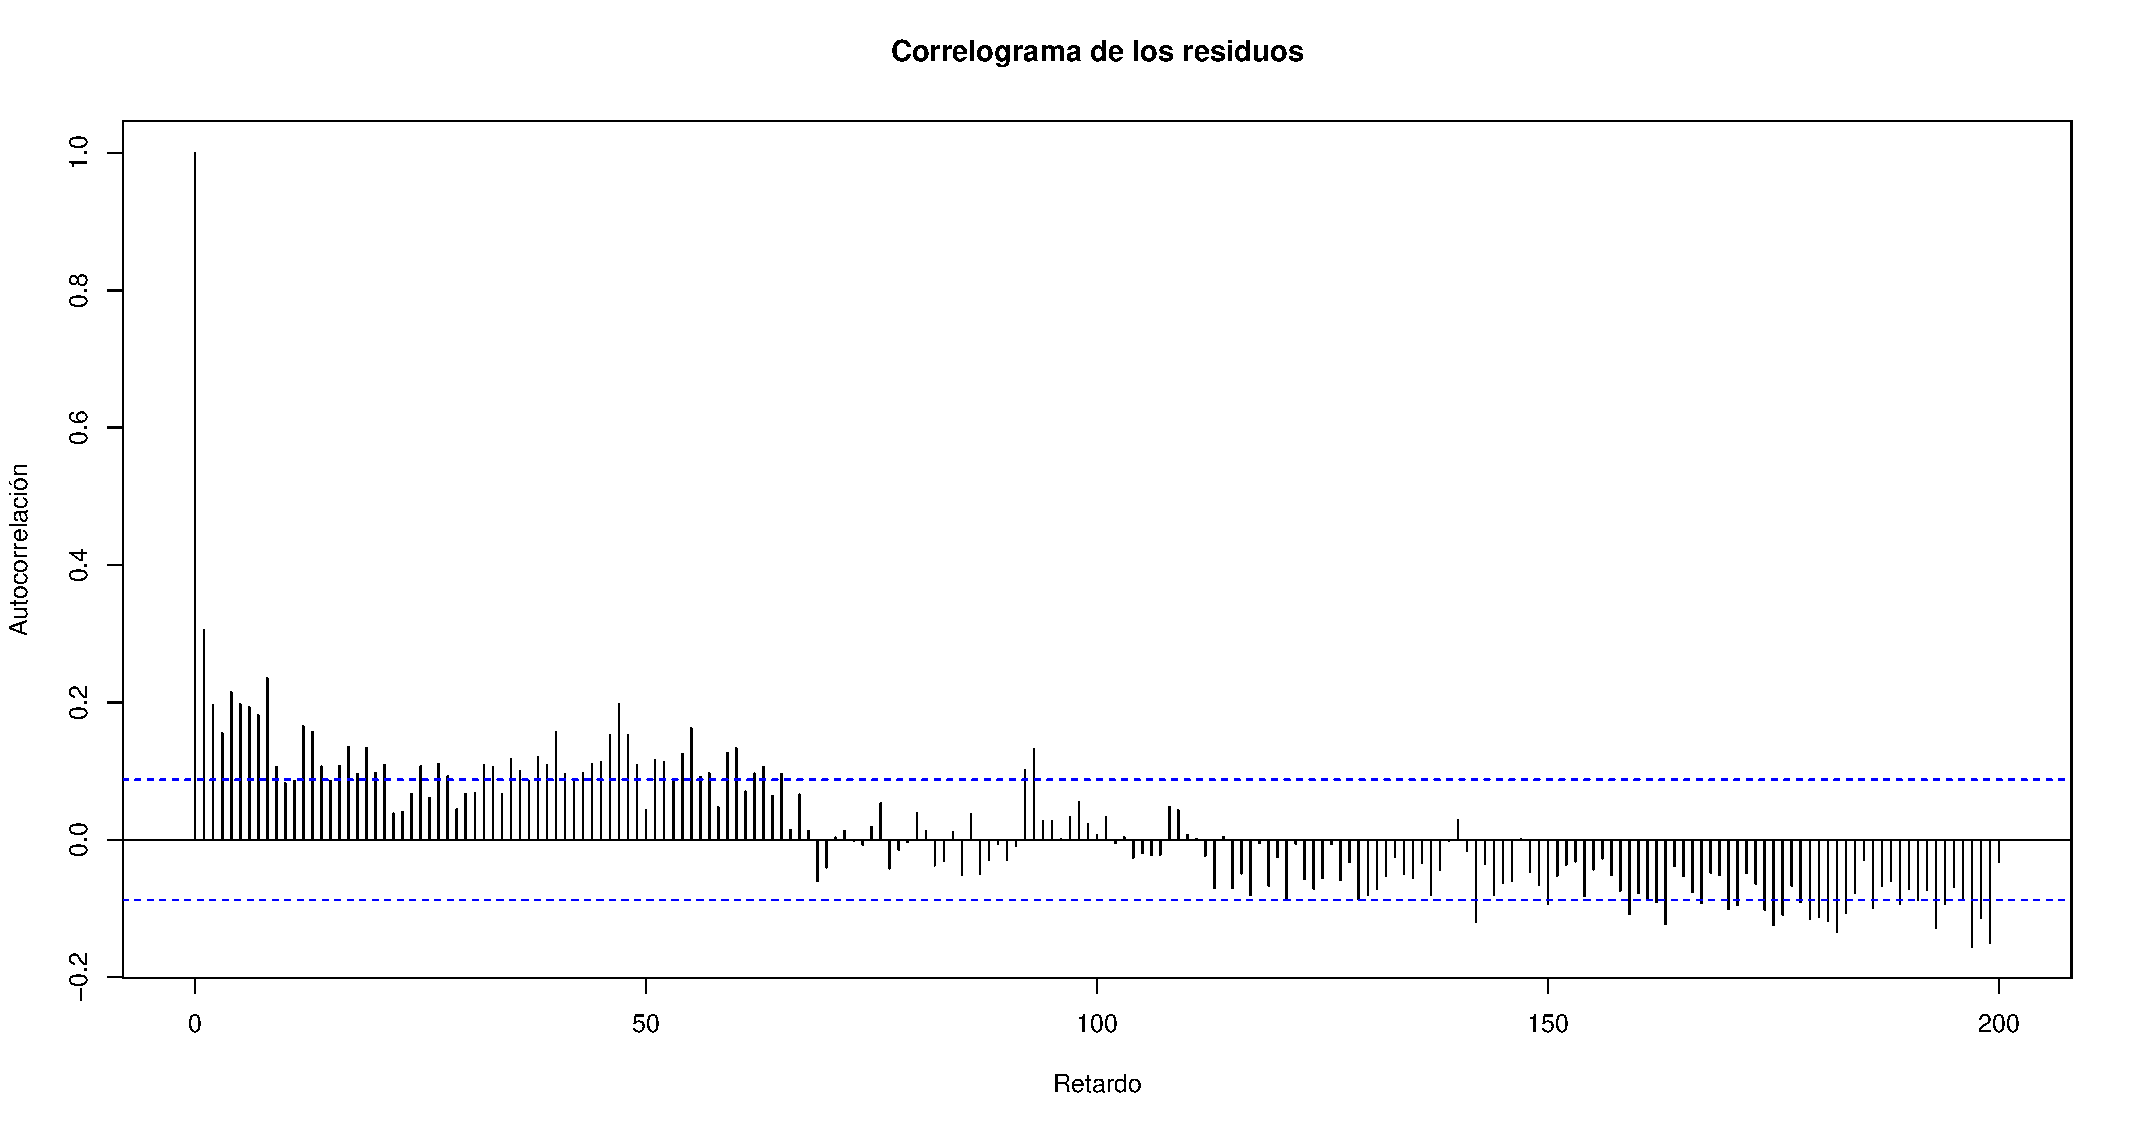
\includegraphics[width=11.8cm]{imagenes/correlograma.pdf}
        \caption{Correlograma de los residuos}
        \label{fig:Densidad}
    \end{center}
\end{figure}
\end{frame}

\begin{frame}
\frametitle{Descripción y resultados de las pruebas aplicadas}
\begin{itemize}
\item Prueba de Rachas:Dada una sucesión de n observaciones de una variable que solo puede tomar dos valores, una racha es una sucesión de uno o más datos con el mismo valor que están seguidos y precedidos por datos con el otro valor, o por ningún dato si se encuentran en el inicio o el final de la sucesión.
~\\ Ejemplo: En la sucesión A BBB AA BB A B se presentan 6 rachas.
~\\ \textbf{Hipótesis:} Las hipótesis que se plantean en esta prueba son:
~\\$H_{0}:$La muestra es aleatoria
~\\$H_{1}:$La muestra no es aleatoria
~\\ \textbf{Estadístico de prueba:} El estadístico de prueba es el número total de rachas, R, en la sucesión.
\end{itemize}
\end{frame}

\begin{frame}
\frametitle{Descripción y resultados de las pruebas aplicadas}
~\\ \textbf{Distribución del estadístico de prueba R:}Su distribución bajo la hipótesis nula $H_{0}$ esta dada por:
~\\$P\left\lbrace{R=r}\right\rbrace=\frac{2\binom{n_{1}-1}{\frac{r}{2}-1}\binom{n_{2}-1}{\frac{r}{2}-1}}{\binom{n_{1}+n_{2}}{n_{1}}}$ si r es par

~\\$P\left\lbrace{R=r}\right\rbrace=\frac{\binom{n_{1}-1}{\frac{r-1}{2}-1}\binom{n_{2}-1}{\frac{r-1}{2}}+\binom{n_{1}-1}{\frac{r-1}{2}}\binom{n_{2}-1}{\frac{r-1}{2}-1}}{\binom{n_{1}+n_{2}}{n_{1}}}$ si r es impar
~\\Para r=2,3,4,...,$n_{1}+n_{2}$
~\\ \textbf{Aproximación a la normal:}
$$Z=\frac{R-\left(\frac{2n_{1}n_{2}}{n_{1}+n_{2}}+1\right)}{\sqrt{\frac{2n_{1}n_{2}(2n_{1}n_{2}-n_{1}-n_{2})}{(n_{1}+n_{2})^2 (n_{1}+n_{2}-1)}}} $$
\end{frame}

\begin{frame}
\frametitle{Descripción y resultados de las pruebas aplicadas}
~\\ \textbf{Región de rechazo:}Se duda de la aleatoriedad cuando hay muchas o muy pocas rachas. Por tanto, la región de rechazo es de la forma:
~\\ $R>R_{n_{1},n_{2};(1-\frac{\alpha}{2})}$ o $R<R_{n_{1},n_{2};\frac{\alpha}{2}}$
~\\Donde la parte derecha de cada inecuación son los percentiles $(1-\frac{\alpha}{2})$ y $\frac{\alpha}{2}$ de la distribución del número de rachas R, cuando hay $n_{1}$ observaciones del tipo A y $n_{2}$ del tipo B.
~\\ \textbf{Resultado:}
\begin{figure}[!h]
    \begin{center}
        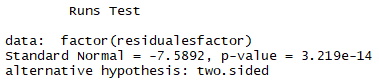
\includegraphics[width=10cm]{imagenes/rachas.png}
        \caption{Resultado prueba de rachas}
        \label{fig:Densidad}
    \end{center}
\end{figure}
\end{frame}

\begin{frame}
\frametitle{Descripción y resultados de las pruebas aplicadas}
\begin{itemize}
\item Prueba de Durbin-Watson: El Test de Durbin-Watson permite evaluar si existe autocorrelación en una Regresión lineal, sea simple o múltiple. Con ello se pretende ver si los valores presentan algún tipo de dependencia en cuanto al orden de obtención. Las hipótesis que se plantean son las siguientes:
~\\$H_{0}:\rho=0$
~\\$H_{1}:\rho\neq 0$
~\\ \textbf{Estadístico de prueba:}El estadístico de Durbin-Watson (D) está condicionado según el orden de las observaciones. El estadístico de Durbin-Watson determina si la correlación entre los términos de error adyacentes es o no es igual a cero. este estadístico esta dado por : $D=\frac{\sum\limits_{t=2}^{n}(e_{t}-e_{t-1})^2}{\sum\limits_{t=1}^{n}e_{t}^2}$ donde $e_{t}$ es el residuo t-esimo o a tiempo t.
\end{itemize}
\end{frame}

\begin{frame}
\frametitle{Descripción y resultados de las pruebas aplicadas}
~\\ \textbf{Región de rechazo:}Para rechazar se utiliza una tabla con lo valores críticos del estadístico, las regiones de rechazo son:
\begin{itemize}
\item Si $d < d_{L,\alpha}$ existe evidencia estadística de que los términos de error estén autocorrelacionados positivamente.
\item Si $d > d_{U,\alpha}$ no hay evidencia estadística de que los términos de error estén autocorrelacionados positivamente.
\item Si $d_{L,\alpha} < d < d_{U,\alpha}$ la prueba no es concluyente.
~\\ \textbf{Resultado:}
\begin{figure}[!h]
    \begin{center}
        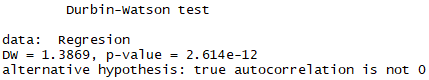
\includegraphics[width=10cm]{imagenes/durbin.png}
        \caption{Resultado de la prueba de Durbin-Watson}
        \label{fig:Densidad}
    \end{center}
\end{figure}
\end{itemize}
\end{frame}

\begin{frame}
\frametitle{Descripción y resultados de las pruebas aplicadas}
\begin{itemize}
\item Prueba de Ljung-Box:La prueba de Ljung-Box es un tipo de prueba estadística que evalúa si un grupo cualquiera de autocorrelaciones de una serie de tiempo son diferentes de cero. En lugar de probar la aleatoriedad en cada retardo distinto, esta prueba la aleatoriedad en general basado en un número de retardos.
~\\En la prueba de Ljung-Box se puede definir o plantear las hipótesis de la siguiente manera:
~\\$H_{0}:$Los datos se distribuyen de forma independiente (es decir, las correlaciones en la población de la que se toma la muestra son 0, de modo que cualquier correlación observada en los datos es el resultado de la aleatoriedad del proceso de muestreo).
~\\$H_{1}:$ Los datos no se distribuyen de forma independiente.
\end{itemize}
\end{frame}

\begin{frame}
\frametitle{Descripción y resultados de las pruebas aplicadas}
~\\ \textbf{Estadístico de prueba:} El estadístico de prueba es: $Q=n(n+2)\sum\limits_{k=1}^{h}\frac{\hat{\rho_{k}^{2}}}{n-k}$
~\\ donde n es el tamaño de la muestra, $\displaystyle {\hat {\rho }}_{k}$  es la autocorrelación de la muestra en el retraso k y h es el número de retardos que se están probando.
~\\ \textbf{Región de rechazo:} Para un nivel de significancia $\alpha$ la región critica para rechazar la hipótesis de aleatoriedad es: $Q>\chi^{2}_{1-\alpha,h}$
~\\donde $\displaystyle \chi _{1-\alpha ,h}^{2}$ es el $\alpha$-cuantil de la distribución chi-cuadrado con m grados de libertad.
\end{frame}

\begin{frame}
\frametitle{Descripción y resultados de las pruebas aplicadas}
~\\ \textbf{Resultado:}\begin{figure}[!h]
    \begin{center}
        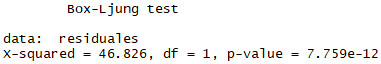
\includegraphics[width=10cm]{imagenes/box.png}
        \caption{Resultado de la prueba de Ljung-Box}
        \label{fig:Densidad}
    \end{center}
\end{figure}
\end{frame}

\begin{frame}
\frametitle{Conclusión sobre nuestro modelo ajustado}
~\\Teniendo en cuenta las pruebas aplicadas, donde vimos que en la prueba gráfica, muchas barras se nos salen de los intervalos y en las pruebas estadísticas los p valores de las tres pruebas son demasiado bajos llevándonos a rechazar siempre $H_{0}$, concluyendo que los residuos no son independientes, lo más común y razonable es concluir que nuestro modelo ajustado no cumple con este supuesto de independencia en los errores, por lo cuál diríamos que lo recomendable sería no usar este modelo. Sin embargo, los errores podrían ser independientes aún cuando los residuos no lo sean, y el supuesto se hace para los errores mas no para los residuos, pero eso no hay forma de probarlo a ciencia cierta, sin embargo hay que tener muy en cuenta los resultados obtenidos y queda a criterio de la persona si ignora estos resultados.
\end{frame}


\end{document}